%%% Hlavní soubor. Zde se definují základní parametry a odkazuje se na ostatní
%%% části. %%%

%% Verze pro jednostranný tisk:
% Okraje: levý 40mm, pravý 25mm, horní a dolní 25mm
% (ale pozor, LaTeX si sám přidává 1in)
\documentclass[12pt,a4paper]{report}
\setlength\textwidth{145mm}
\setlength\textheight{247mm}
\setlength\oddsidemargin{15mm}
\setlength\evensidemargin{15mm}
\setlength\topmargin{0mm}
\setlength\headsep{0mm}
\setlength\headheight{0mm}
% \openright zařídí, aby následující text začínal na pravé straně knihy
\let\openright=\clearpage

%% Použité kódování znaků: obvykle latin2, cp1250 nebo utf8:
\usepackage[utf8]{inputenc}

%% Ostatní balíčky
\usepackage{graphicx}
\usepackage{amsthm}
\usepackage{amsmath}
\usepackage{mathtools}
\usepackage{gnuplottex}

%% Balíček hyperref, kterým jdou vyrábět klikací odkazy v PDF,
%% ale hlavně ho používáme k uložení metadat do PDF (včetně obsahu).
%% POZOR, nezapomeňte vyplnit jméno práce a autora.
\usepackage[ps2pdf,unicode]{hyperref}   % Musí být za všemi ostatními balíčky
\hypersetup{pdftitle=Fast and Trainable Tokenizer for Natural Languages}
\hypersetup{pdfauthor=Jiří Maršík}

%%% Drobné úpravy stylu

% Tato makra přesvědčují mírně ošklivým trikem LaTeX, aby hlavičky kapitol
% sázel příčetněji a nevynechával nad nimi spoustu místa. Směle ignorujte.
\makeatletter
\def\@makechapterhead#1{
  {\parindent \z@ \raggedright \normalfont
   \Huge\bfseries \thechapter. #1
   \par\nobreak
   \vskip 20\p@
}}
\def\@makeschapterhead#1{
  {\parindent \z@ \raggedright \normalfont
   \Huge\bfseries #1
   \par\nobreak
   \vskip 20\p@
}}
\makeatother

% Toto makro definuje kapitolu, která není očíslovaná, ale je uvedena v obsahu.
\def\chapwithtoc#1{
\chapter*{#1}
\addcontentsline{toc}{chapter}{#1}
}

\usepackage{mystyle}

\begin{document}

% Trochu volnější nastavení dělení slov, než je default.
\lefthyphenmin=2
\righthyphenmin=2


%%% Titulní strana práce

\pagestyle{empty}
\begin{center}

\large

Charles University in Prague

\medskip

Faculty of Mathematics and Physics

\vfill

{\bf\Large BACHELOR THESIS}

\vfill

\centerline{\mbox{
\includegraphics[width=60mm]{img/logo.eps}}}

\vfill
\vspace{5mm}

{\LARGE Jiří Maršík}

\vspace{15mm}

% Název práce přesně podle zadání
{\LARGE\bfseries Fast and Trainable Tokenizer \\ for Natural Languages}

\vfill

% Název katedry nebo ústavu, kde byla práce oficiálně zadána
% (dle Organizační struktury MFF UK)
Institute of Formal and Applied Linguistics

\vfill

\begin{tabular}{rl}

Supervisor of the bachelor thesis: & RNDr. Ondřej Bojar, Ph.D. \\
\noalign{\vspace{2mm}}
Study program: & Computer Science \\
\noalign{\vspace{2mm}}
Specialization: & General Computer Science \\
\end{tabular}

\vfill

% Zde doplňte rok
Prague 2011

\end{center}

\newpage

%%% Následuje vevázaný list -- kopie podepsaného "Zadání bakalářské práce".
%%% Toto zadání NENÍ součástí elektronické verze práce, nescanovat.

%%% Na tomto místě mohou být napsána případná poděkování (vedoucímu práce,
%%% konzultantovi, tomu, kdo zapůjčil software, literaturu apod.)

\openright

\noindent
Dedicated to the work of B\'ela Tarr.

\newpage

%%% Strana s čestným prohlášením k bakalářské práci

\vglue 0pt plus 1fill

\noindent
I declare that I carried out this bachelor thesis independently, and only with
the cited sources, literature and other professional sources.

\medskip\noindent
I understand that my work relates to the rights and obligations under the Act
No. 121/2000 Coll., the Copyright Act, as amended, in particular the fact that
the Charles University in Prague has the right to conclude a license agreement
on the use of this work as a school work pursuant to Section 60 paragraph 1 of
the Copyright Act.

\vspace{10mm}

\hbox{\hbox to 0.5\hsize{%
In ........ date ............
\hss}\hbox to 0.5\hsize{%
signature
\hss}}

\vspace{20mm}
\newpage

%%% Povinná informační strana bakalářské práce

\vbox to 0.5\vsize{
\setlength\parindent{0mm}
\setlength\parskip{3mm}

\begin{singlespace}
\begin{otherlanguage}{czech}

Název práce:
Rychlý a trénovatelný tokenizér pro přirozené jazyky
% přesně dle zadání

Autor:
Jiří Maršík

Katedra:  % Případně Ústav:
Ústav formální a aplikované lingvistiky
% dle Organizační struktury MFF UK

Vedoucí bakalářské práce:
RNDr. Ondřej Bojar Ph.D.
% dle Organizační struktury MFF UK, případně plný název pracoviště mimo MFF UK

Abstrakt:
% abstrakt v rozsahu 80-200 slov; nejedná se však o opis zadání bakalářské
% práce
V této práci představujeme systém pro dezambiguaci hranic mezi tokeny a větami.
Charakteristickým znakem programu je jeho značná konfigurovatelnost a
všestrannost, tokenizér si dokáže poradit např. i s nepřerušovaným čínským
textem. Tokenizér používá klasifikátory založené na modelech s maximální
entropií a jedná se tudíž o systém strojového učení, kterému je nutné předložit
již tokenizovaná data k trénování. Program je doplněn nástrojem pro hlášení
úspěšnosti tokenizace, což pomáhá zejména při rychlém vývoji a ladění
tokenizačního procesu. Systém byl vyvinut pouze za pomoci multiplatformních
knihoven a při vývoji byl kladen důraz zejména na efektivitu a správnost. Po
nezbytném přehledu jiných tokenizérů a krátkém úvodu do teorie modelů s
maximální entropií se většina textu práce zabývá vlastní implementací
tokenizéru a vyhodnocením jeho úspěšnosti.

Klíčová slova:
tokenizace, segmentace, maximální entropie, předzpracování textu
% 3 až 5 klíčových slov

\end{otherlanguage}
\end{singlespace}

\vss}\nobreak\vbox to 0.49\vsize{
\setlength\parindent{0mm}
\setlength\parskip{3mm}

\begin{singlespace}

Title:
Fast and Trainable Tokenizer for Natural Languages
% přesný překlad názvu práce v angličtině

Author:
Jiří Maršík

Department:
Institute of Formal and Applied Linguistics
% dle Organizační struktury MFF UK v angličtině

Supervisor:
RNDr. Ondřej Bojar Ph.D.
% dle Organizační struktury MFF UK, případně plný název pracoviště
% mimo MFF UK v angličtině

Abstract:
In this thesis, we present a data-driven system for disambiguating token and
sentence boundaries. The implemented system is highly configurable and
versatile to the point its tokenization abilities are able to satisfactorily
segment unbroken Chinese text. The tokenizer relies on maximum entropy
classifiers and requires tokenized and segmented text as training data. The
program is accompanied by a tool for reporting the performance of the
tokenization which helps to rapidly develop and tune the tokenization process. The
system was built with multi-platform libraries only and with emphasis on speed
and correctness. After a necessary survey of other tools for text tokenization
and segmentation and a short introduction to maximum entropy modelling a large
part of the thesis focuses on the particular implementation we developed and
its evaluation.
% abstrakt v rozsahu 80-200 slov v angličtině; nejedná se však o překlad zadání
% bakalářské práce

Keywords:
% 3 až 5 klíčových slov v angličtině
tokenization, segmentation, maximum entropy, text preprocessing

\end{singlespace}

\vss}

\newpage


\openright
\pagestyle{plain}
\setcounter{page}{1}

%%% Jednotlivé kapitoly práce jsou pro přehlednost uloženy v samostatných
%%% souborech
\chapter*{Introduction}
\addcontentsline{toc}{chapter}{Introduction}

The goal of this thesis was to provide a fast implementation of a system for
disambiguating token and sentence boundaries and to evaluate the
implementation both in terms of its accuracy and its speed.

Token and sentence boundary disambiguation may seem trivial at first, and it
usually is, but in some occasions it might turn out to be quite complex.
Consider the following cases:

\begin{exe}
  \ex{\label{ex:long-context-a}
      On Friday, the 22\textsuperscript{nd}, at around 2 a.m.\ Dr.~T.~Adams
      finished the preliminary examination.}
  \ex{\label{ex:long-context-b}
      The field tests were to begin on Friday, the 22\textsuperscript{nd}, at
      around 2 a.m. Dr.~T.~Adams finished the preliminary examination the night
      before.}
  \ex{"314 159.26\$, about half of the yearly budget, was spent on office
      redecoration!", protested the disgruntled employee of Vanity, S.p.A\@.}
\end{exe}

Even as I was typesetting these examples in \LaTeX{}, I had to explicitly mark
some of the periods in the above examples as not being sentence boundaries, as
\LaTeX{} likes to instert slighly larger spaces after sentence terminators (so
called French spacing). The heuristic used by \LaTeX{} is very simple: if a
word-final potential sentence terminator (a period, a question mark or an
exclamation mark) follows a capital letter, then it is most likely a part of
an abbreviation (or an initial) and so it does not mark the end of a
sentence\footnote{TODO: viz.mail} \cite{web-latex}.

Such a simple system runs into problems in the examples given above, as we
can see that abbreviations do not necessarily end with capital letters and on
top of that a period may serve both as part of an abbreviation and a sentence
terminator. Examples \ref{ex:long-context-a} and \ref{ex:long-context-b} also
show us that the context needed to disambiguate the sentence boundary may be
quite far from the boundary in question.

While getting the size of a space correctly down to the last millimeter is
certainly a noble goal, there are also some important uses for a more reliable
segmenter and tokenizer. When text is being processed and parsed by automatic
tools, a common first step is to divide the text into tokens and sentences. A
lot of the tools that then work with these tokens assume they are correct and
try to analyze them further. As a lot of these tools are getting more and more
accurate, it is important we step up the quality of the tokenization process,
so that the system's quality is not determined by something as basic as
tokenization and segmentation of input. 

In the last 20 years, the problem started getting some recognition and several
systems were demonstrated. This thesis does not aim to create a new system for
tokenization. This work is based on an already existing tokenizer implemented
by Ondřej Bojar during the construction of the UMC 0.1 Czech-Russian-English
Multilingual Corpus \cite{maxent-original-paper,maxent-original}.

A key feature of the original tokenizer is its strict segregation of
language-dependent knowledge into configurable files. The new implementation
expands on this idea and assumes next to nothing about the language being
processed except that the sentence and token boundaries are disambiguated by a
limited context window described by binary predicates expressed as regular
expressions. The tokenizer thus offers a great deal of customizability and a
lot of effort has been put into ensuring that the tokenizer will behave as
expected and that the behaviour is easy to understand without diverging too
much from the original.

Performance, being the motivation behind the current implementation, was also
important. Both the original and the new tokenizer rely on a C++ toolkit which
handles the mechanics of machine learning \cite{maxent-toolkit}. However, the
original implementation, being written in Perl, had to access the functionality
through a command-line interface passing data through files. The new
implementation will have the benefits of using the C++ API directly. Where the
old implementation used regular expressions to partition the input and detect
potential token and sentence boundaries, the new implementation uses a lexical
analyzer generator \cite{web-quex} to generate fast C++ code, compile it and
load it at runtime. The new implementation also benefits from the multiple CPUs
found on modern computers and uses a high-level parallelism library
\cite{web-tbb} to perform the various time-consuming tasks of tokenization in
parallel.

In Chapter~\ref{chap:survey}, we will look at other systems which tried to
tackle the problem and compare them to our tokenizer. In
Chapter~\ref{chap:maxent}, a brief overview of the maximum entropy method of
machine learning will be given. Chapter~\ref{chap:impl} will familiarize us
with the implementation of the tokenizer. Finally, in Chapter~\ref{chap:eval},
we evaluate the speed and accuracy of the tokenizer on several datasets.

\chapter{A Survey of Other Solutions}
\label{chap:survey}

Placeholder text?

\section{RE}
\label{sec:survey-re}

The system referred to as RE in [] is an example of a purely
\newterm{rule-based} system. It does not need any training data, but instead it
relies on explicit linguistic knowledge such as lists of abbreviations and
custom regular expressions. The RE system in particular works by scanning the
input text for periods and then inspecting the tokens surrounding it. If the
surrounding tokens do not match a combination of the user's regular
expressions, the period is marked as a sentence boundary.

Our tokenizer also allows the user to define regular expressions against which
neighboring tokens will be checked (not only neighboring tokens, a token at any
distance can be examined, which can be important as we saw in the
introduction). The crucial difference between the RE system and our tokenizer
is that the outcomes of all these regular expression tests are not explicitly
mapped to the disambiguation of the potential boundary by the programmer or the
user. Instead, our system relies on already tokenized data from which it learns
how to combine the outcomes of these regular expression tests into a
tokenization decision.

\section{MxTerminator}
\label{sec:survey-mxterm}

Contrary to RE, MxTerminator is a \newterm{supervised machine-learning} system.
This means that the tool has to be supplied with already tokenized data from
which the classifier infers the logic behind tokenization. The classifier in
this case is based on maximum entropy models, the same mathematical foundation
on which our system is built.

The MxTerminator scans the text for a list of potential sentence terminators
and presents the classifier with features of the neighboring tokens. The
features include the word containing the potential sentence terminator, the
words preceding and following it, the presence of particular characters in the
current word and whether the current word is a honorific or a corporate
designator (e.g.\ Corp.). All of these are easily expressed using regular
expressions and lists of tokens and so it should be quite easy to produce a
system very similar to MxTerminator using a specific configuration.

There is also a more general version of the MxTerminator which does not rely on
precompiled lists of honorifics and other abbreviations. In this version, the
MxTerminator first scans the training data and searches for words containing a
period which does not serve as a sentence terminator. The features passed to
the maximum entropy classifier then consist only of the trigram of words
containing the potential sentence terminator and values describing whether the
individual words belong to the abbreviations induced from training data in the
previous step. With our tokenizer it is also possible to scan the training data
and extract a list of induced abbreviations. These can then be stored in a
token list and the tokenizer can be configured to check whether tokens are in
that list and pass the result to the classifier.

\section{Riley}
\label{sec:survey-riley}

Riley uses a method of classification different from the MxTerminator. Instead
of using a maximum entropy classifier, he builds a regression tree. The
following features are used to disambiguate the period (let $a$ be the word
containing the period in question and $b$ the following word):

\begin{itemize}
  \item Probability of $a$ occuring at the end of a sentence
  \item Probability of $b$ occuring at the beginning of a sentence
  \item Length of $a$
  \item Length of $b$
  \item Case of $a$
  \item Case of $b$
  \item Any punctuation after the period
  \item Abbreviation class of $a$
\end{itemize}

A training dataset the size of approximately 25 million words was used to
estimate the probabilities of individual words occuring near sentence
boundaries. Thanks to such detailed information, the system was found to
perform notably well.

The first two features used in the regression tree have a natural counterpart
in the maximum entropy model. When the text of a token is being passed to the
maximum entropy classifier during training, it estimates a parameter for each
type of token encountered and each possible outcome (no boundary, token
boundary, sentence boundary). What this parameter does, basically, is that it
describes and retains in the model the probability of encountering a specific
token together with a specific outcome. The equivalent of a probability of a
certain token occuring near the sentence boundary would therefore be the
maximum entropy model's parameter corresponding to the event of that token
appearing together with the sentence boundary outcome.

As for the length features, our tokenizer uses a more general form of a maximum
entropy feature which allows for real feature values instead of only binary
(the only such feature in use, however, is the built-in length of a token).
The remaining parameters can be described by binary features defined as regular
expressions supplied by the user.

\section{Satz}
\label{sec:survey-satz}

The Satz system is another supervised machine-learning system for sentence
boundary disambiguation. It is very unique in that it does not rely on the
superficial characteristics of the shape of the surrounding tokens. Instead, it
passes to the underlying classifier the probability distribution of parts of
speech for every token within the context of the potential sentence boundary.
It is therefore necessary to supply a lexicon giving the part of speech
distribution. If a word is not part of any lexicon, a series of heuristics try
to guess a safe probability distribution given the word's suffix, case,
internal punctuation etc... Thanks to the generalization provided by the part
of speech categories, the system required relatively small amounts of training
data to acheive solid performance.

In our system, the user is limited to defining binary features and so passing
the probability distributions to the classifier would be out of the question.
However, the authors of the Satz system performed an experiment wherein they
replaced the non-zero probabilities with ones (basically switching from part of
speech probabilities to flags indicating if a given part of speech is
possible). The results of this experiment showed that the resulting system was
trained faster and performed better than the original. Luckily our tokenizer
allows the user to easily define binary features using lists of tokens, i.e.\
lexicons. The only problem would be the heuristics employed with out of
vocabulary words. While all of them can be easily expressed as regular
expressions in our system, there is yet no mechanism to make the tokenizer
treat a part of speech found in a lexicon and a part of speech guessed by a
heuristic as the same feature.


\chapter{Implementation}
\label{chap:impl}

In this chapter we describe the internal design of the tokenizer and provide
rationale for the choices behind it. We explore the problem of rough
tokenization more deeply as it posed one the biggest challenges in building the
system. Finally, we talk about the multi-threading tools which were used to
enable parallelism in the tokenizer.

\section{Overview of the System}
\label{sec:impl-overview}

The data flow between the various subsystems can be seen in
figure~\ref{fig:all-parts}.

\begin{figure}[ht]
  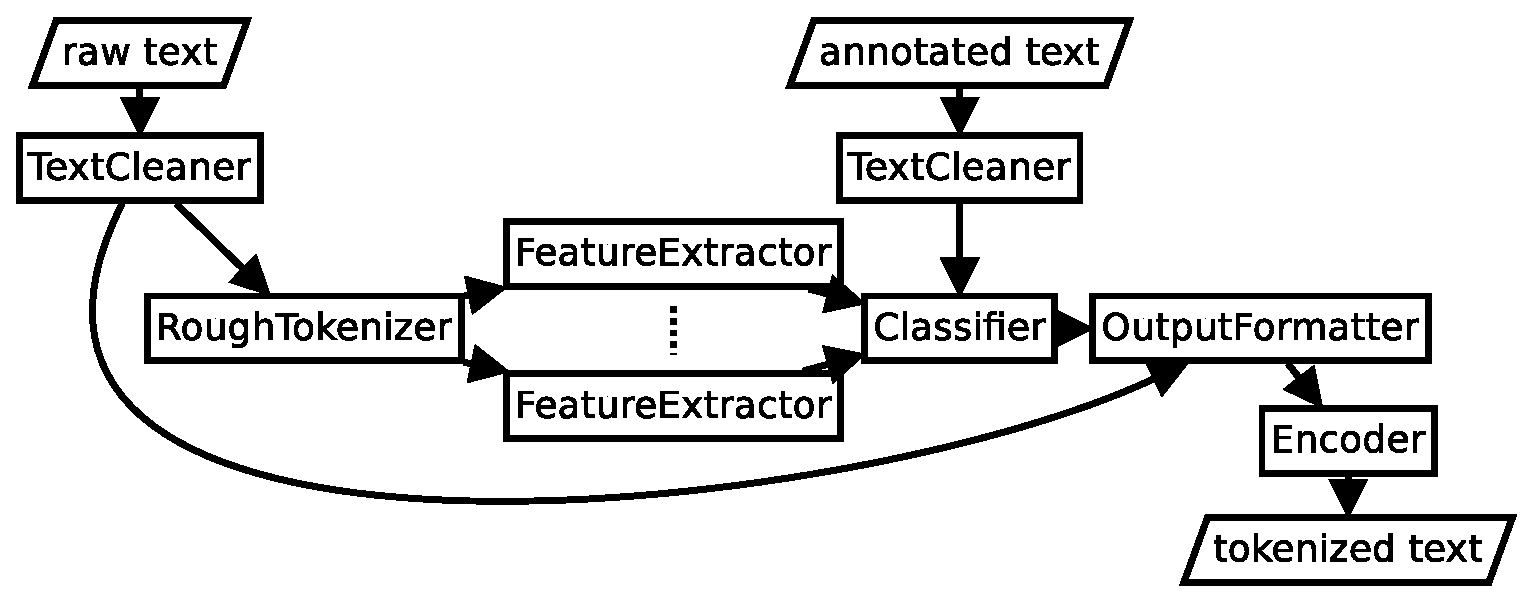
\includegraphics[width=\textwidth]{img/all-parts.eps}
  \caption{Data flow in the entire system}
  \label{fig:all-parts}
\end{figure}

\subsection{TextCleaner}

Any input which is read by the tokenizer is first processed with the
TextCleaner. This unit is responsible for decoding the stream of text and
optionally removing XML markup and expanding HTML entities and character
references. These changes to the input stream (referred to as cutouts in the
program) are conveyed to the OutputFormatter so that they can be undone in the
output. This allows the tokenizer to process XML marked up content as if it was
plaintext. The XML markup thus cannot be broken by and does not interfere with
the tokenization process.

\subsection{RoughTokenizer}

The RoughTokenizer's goal is to examine the cleaned input stream and identify
both unambiguous and ambiguous token and sentence boundaries. It does so by
splitting the text into what we call rough tokens. In the simplest case, rough
tokens are the whitespace delimited words of the text (the term word will be
used to mean a maximal subsequence of nonwhite characters). However, the user
can write regular expressions to define certain points within and between these
strings of nonwhite characters which may split them up into what end up being
the rough tokens. These user-defined points are called decision points and they
represent the ambiguous token/sentence boundaries.

There are three types of decision points. There is the MAY\_SPLIT which occurs
within words and signals a potential token boundary. The MAY\_BREAK\_SENTENCE
occurs before and after certain characters and marks a potential sentence
boundary. MAY\_SPLIT and MAY\_BREAK\_SENTENCE are the decision points which
split words into rough tokens. The third type of decision point is MAY\_JOIN
which occurs between words and turns the space between them from a token
boundary to a potential token boundary, making it possible for the two words to
join into a single token.

The rough tokenizer detects all decision points in the text and produces a
stream of discrete rough tokens annotated with information about surrounding
whitespace and decision points.

\subsection{FeatureExtractor}



\chapter{Evaluation}
\label{chap:eval}

\chapter*{Conclusion}
\addcontentsline{toc}{chapter}{Conclusion}

We have presented a data-driven system for tokenizing and segmenting text. We
have demonstrated the system's versatility by combining methods based on
different techniques such as morphological dictionaries, regular expressions
and exception lists. The system proved its universal applicability in being
able to act both as a sentence boundary disambiguator for languages such as
English and Czech and as a word segmenter for languages which do not use
whitespace such as Chinese. We have also pointed to the fact that the program
relies only on multiplatform programs and libraries. While it has not been
tested on Windows or MacOS yet, care was taken at every step to ensure it would
be a smooth transition (ICU can be used instead of libiconv for character code
conversion, CMake is used for building, OS-specific matters are accessed via
Boost only\ldots).

We measured the accuracy, precision, recall and F-measure of the token and
sentence boundary disambiguation. The tests were executed with several very
different tokenization schemes and on several datasets in multiple languages.
We also measured and analyzed the tokenizer's speed and identified the
bottleneck which should serve as an avenue for further optimization.

The natural next step would be to invent and experiment with new ways and
features for tokenizing and segmenting text. The system offers fast feedback on
the accuracy of the user's tokenization schemes and is helpful in pointing out
positions in the text which are yet to be covered by rules for inserting
decision points. Another possible elaboration might be to change the maximum
entropy training backend to the Toolkit for Advanced Discriminative Modelling
or some other alternative.


%%% Seznam použité literatury

% Here I \nocite all the original sources.
\nocite{web-cmake}
\nocite{web-libtool}
\nocite{web-tbb}
\nocite{web-latex}
\nocite{web-openmp}
\nocite{web-pcre}
\nocite{web-re2}
\nocite{maxent-approach}
\nocite{web-nltk}
\nocite{maxent-original}
\nocite{web-boost}
\nocite{web-bakeoff}
\nocite{sbd-re}
\nocite{sbd-punkt}
\nocite{maxent-original-paper}
\nocite{maxent-toolkit}
\nocite{seg-chinese-maxent}
\nocite{maxent-algorithms}
\nocite{web-tadm}
\nocite{web-pipes}
\nocite{sbd-satz}
\nocite{web-stanford}
\nocite{maxent-simple}
\nocite{sbd-mxterm}
\nocite{sbd-riley}
\nocite{web-quex}

\bibliographystyle{iso690}
\cleardoublepage
\phantomsection
\addcontentsline{toc}{chapter}{Bibliography}
\bibliography{sbd,maxent,seg,web}

\openright
\end{document}
